 \setlength{\baselineskip}{20pt}
\chapter{第二章:一级标题}
\label{cha:chap2}

[鼠标左键单击选择该段落,输入替换之。内容为小四号宋体。] 学位论文为了需要反映出作者确已掌握了坚实的基础理论和系统的专门知识,具有开阔的科学视野,对研究方案作了充分论证,因此,有关历史回顾和前人工作的综合评述,以及理论分析等,可以单独成章,用足够的文字叙述。正文是学位论文的核心部分,占主要篇幅,可以包括:调查对象、实验和观测方法、仪器设备、材料原料、实验和观测结果、计算方法和编程原理、数据资料、经过加工整理的图表、形成的论点和导出的结论等。


由于研究工作涉及的学科、选题、研究方法、工作进程、结果表达方式等有很大的差异,对正文内容不能作统一的规定。但是,必须实事求是,客观真切,准确完备,合乎逻辑,层次分明,简练可读。


\textbf{图}:见《北京交通大学学位论文撰写规范》3.10.4
\begin{figure}[!htb] % use float package if you want it here
%\setlength{\abovecaptionskip}{-0.2cm} %调整图片caption与正文之间的间距,table同理。可自己调整。
\setlength{\belowcaptionskip}{-0.2cm} 
  \centering
  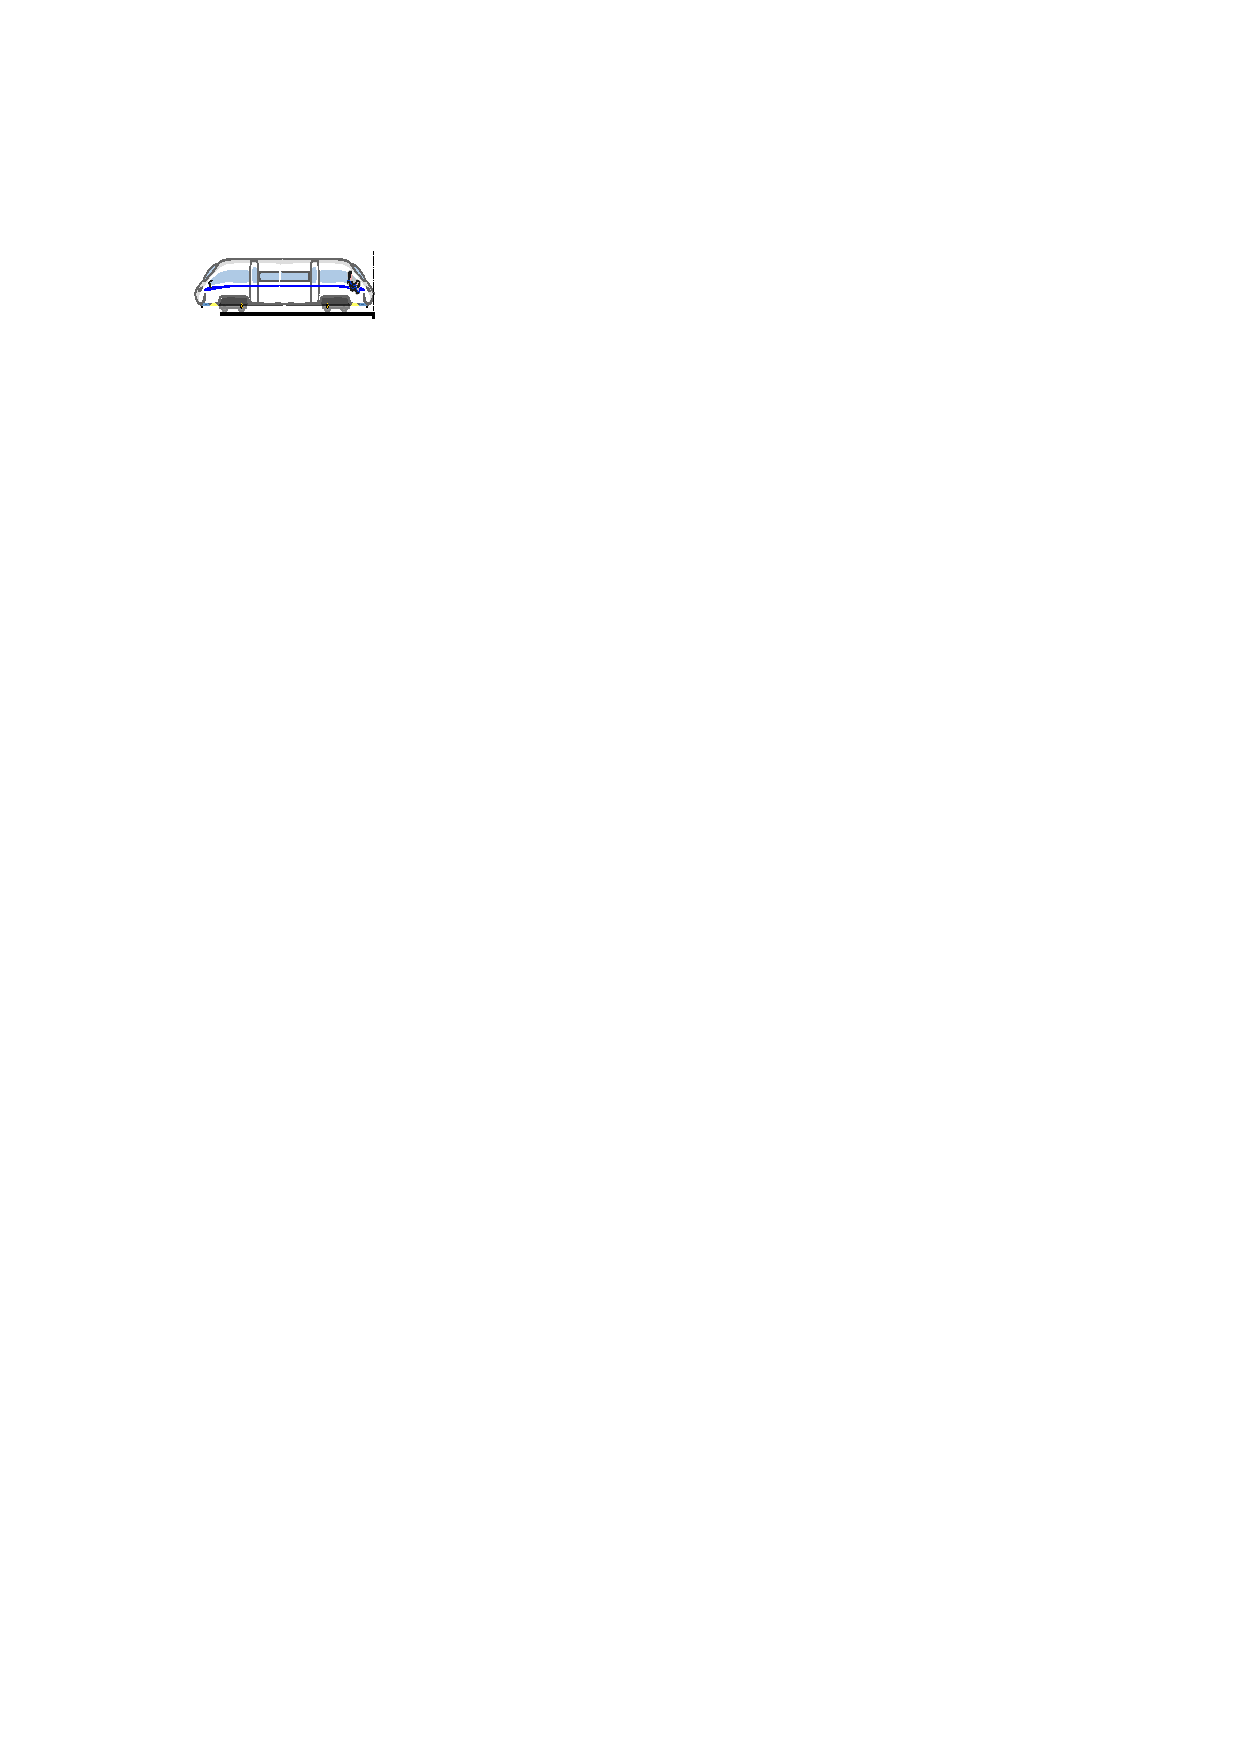
\includegraphics[scale=1]{figures/figure1.pdf}
  \caption{示例图片。\\Fig~\ref{fig:02:01}~Example of Figure.}
  \label{fig:02:01}
\end{figure}

图应有编号。图的编号由“图”和从“1”开始的阿拉伯数字组成,图较多时,可分章依序编号。

图宜有图题,图题即图的名称,置于图的编号之后。图的编号和图题应置于图下方。图题采用中英文对照,英文(Times New Roman)字体五号,中文宋体五号。居中书写,中文在上。

照片图要求主题和主要显示部分的轮廓鲜明,便于制版。如用放大缩小的复制品,必须清晰,反差适中。照片上应有表示目的物尺寸的标度。

例如:如图\ref{fig:02:01}所示
\begin{figure}[h]
%\setlength{\abovecaptionskip}{-0.2cm} %调整图片caption与正文之间的间距,table同理。可自己调整。
\setlength{\belowcaptionskip}{-0.2cm} 
 \centering
 \addtocounter{subfigure}{-1}\subfigure[English caption1] {\subfigure[中文标题1] { 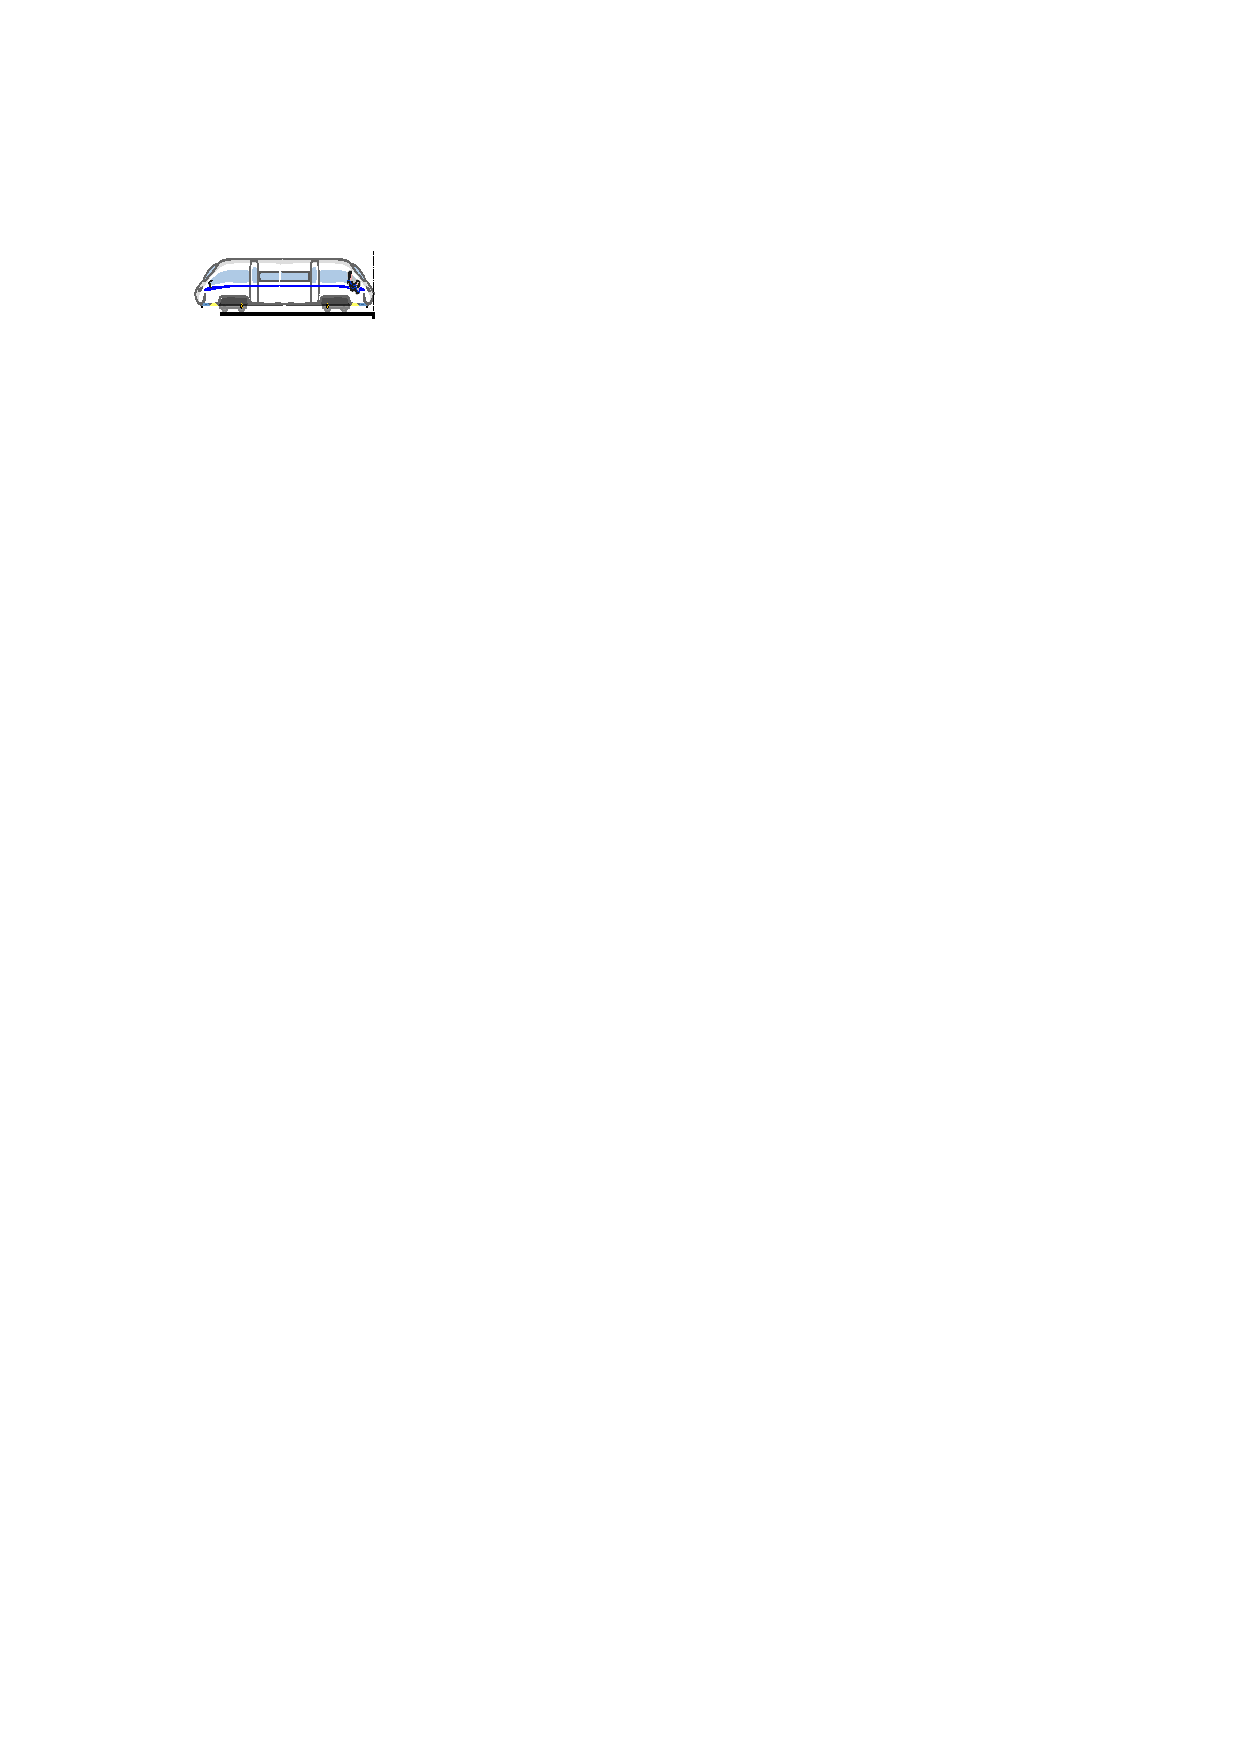
\includegraphics[scale=1]{figures/figure1.pdf}}}
 \addtocounter{subfigure}{-1}\subfigure[English caption2] {\subfigure[中文标题2]{ 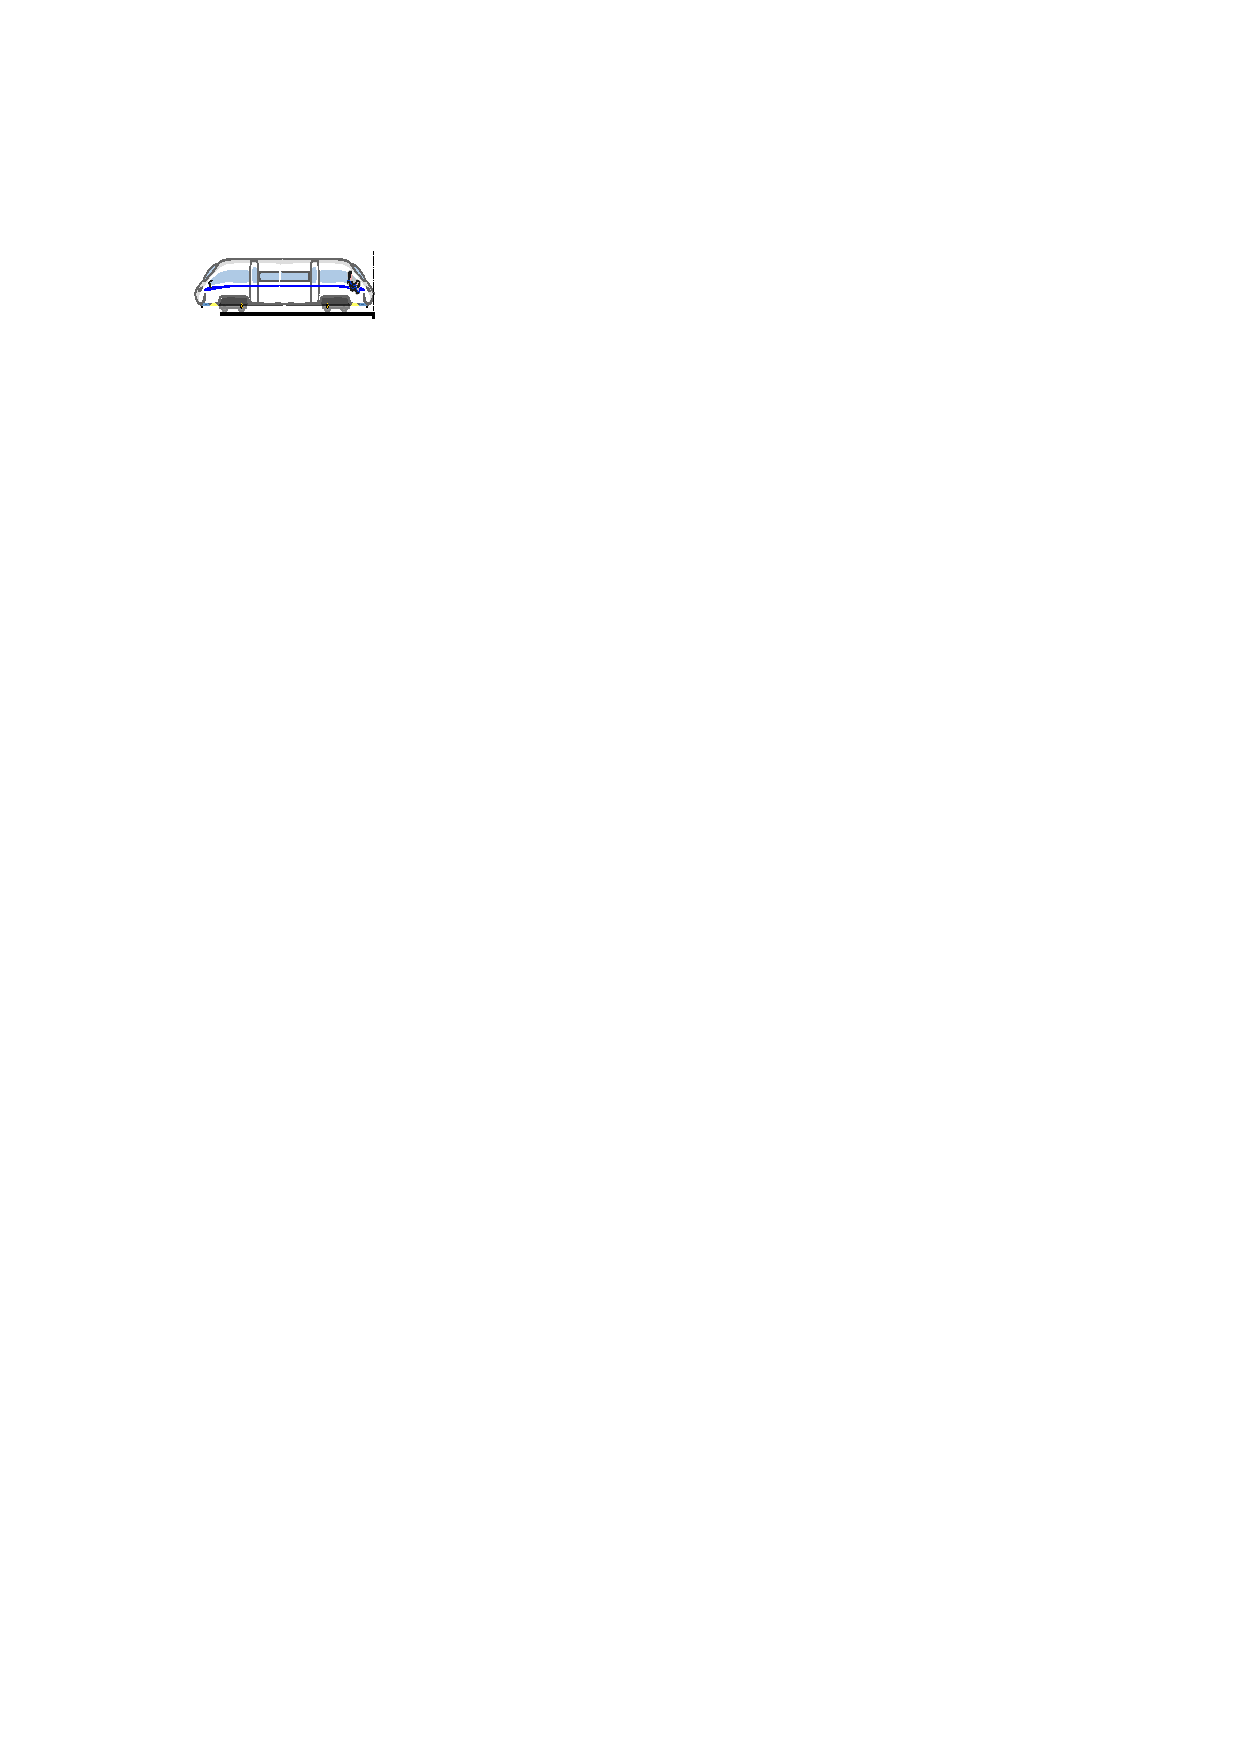
\includegraphics[scale=1]{figures/figure1.pdf}}}
 \caption{示例图片。\\Fig~\ref{fig:02:02}~Example of Figure.}
 \label{fig:02:02}
  \end{figure} 

\textbf{表}:见《北京交通大学学位论文撰写规范》3.10.5

表应有编号。表的编号由“表”和从“1”开始的阿拉伯数字组成,表较多时,可分章依序编号。

表宜有表题,表题即表的名称,置于表的编号之后。表的编号和表题应置于表上方。表题采用中英文对照,居中,中文在上。英文(Times New Roman)字体五号,中文宋体五号。

表的编排,一般是内容和测试项目由左至右横读,数据依序竖读。
表的编排建议采用国际通行的三线表。

如某个表需要转页接排,在随后的各页上应重复表的编号。编号后跟表题(可省略)和“(续)”,置于表上方。
续表均应重复表头。

例如:如表格\ref{table:02:01}所示

\begin{table}[!htb]\small   %%\small是为了设置表格中的字体比正文小
\setlength{\abovecaptionskip}{-0.05cm} %调整图片caption与正文之间的间距,table同理。可自己调整。
\setlength{\belowcaptionskip}{-0.2cm} 
  \centering
  \renewcommand\arraystretch{1}
  \caption{示例表格。\\Table~\ref{table:02:01}~Example of Table.}

 \begin{tabular}{p{1cm} p{1cm}<{\centering} p{1cm}<{\centering} p{1cm}<{\centering} p{1cm}<{\centering} p{1cm}<{\centering}  }
  \hline
  \textbf{AA} &
  \textbf{BB} &
  \textbf{CC} &
  \textbf{DD} &
  \textbf{EE} &
  \textbf{FF}
  \\
  \hline
    AA   &  1.1   & 1.1 & 1.1 & 1.1&  1.1    \\
    BB   &  1.1   & 1.1 & 1.1 & 1.1&  1.1    \\
    CC   &  1.1   & 1.1 & 1.1 & 1.1&  1.1   \\
  \hline
  \end{tabular}
  \label{table:02:01}
\end{table}


\textbf{公式}:见《北京交通大学学位论文撰写规范》3.10.12

论文中的公式应另行起,并居中书写,与周围文字留足够的空间区分开。

如有两个以上的公式,应用从“1”开始的阿拉伯数字进行编号,并将编号置于括号内。公式的编号右端对齐,公式与编号之间可用“…”连接。公式较多时,可分章编号。

较长的公式需要转行时,应尽可能在“$ = $”处回行,或者在“$ + $”、“$-$”“$*$”等记号处回行。公式中分数线的横线,其长度应等于或略大于分子和分母中较长的一方。
如正文中书写分数,应尽量将其高度降低为一行。如将分数线书写为“$/$”,将根号改为负指数。


单独为行公式示例:如公式\ref{eq:02:01},公式\ref{eq:02:02a}所示。

\begin{equation}\label{eq:02:01}
\left\{
\begin{split}
\frac{\texttt{d}p(t)}{\texttt{d}t}&=v(t)\\
\frac{\texttt{d}v(t)}{\texttt{d}t}&=u(t)-a(t)-b(t)v(t)-c(t)v^2(t)-f_2^*(\cdot)
\end{split}
\right.
\end{equation}


\begin{subequations}\label{eq:02:02}
  \begin{align}
  \dot{\hat{A}}^\dag&=\lambda_1\left(\tanh(k_3e_v)e_v-\sigma_1\hat{A}^\dag\right)\label{eq:02:02a}\\
  \dot{\hat{b}}^\dag&=\lambda_2\left(|v||e_v|-\sigma_2\hat{b}^\dag\right)\label{eq:02:02b}\\
  \dot{\hat{c}}^\dag&=\lambda_3\left(v^2|e_v|-\sigma_3\hat{c}^\dag\right)\label{eq:02:02c}
  \end{align}
  \end{subequations}

嵌入在文本中的公式例子:$a + b = c$。



\textbf{引用}:见《北京交通大学学位论文撰写规范》3.10.7
论文中引用的文献的标注方法遵照GB/T 7714-2005,采用顺序编码制,并以参考文献形式统一编号。正文中引用文献的标示应置于所引内容最后一个字的右上角,所引文献编号用阿拉伯数字置于方括号“[ ]”中,用小4号字体的上角标。

例如,引用参考文献\cite{MATSUMURA2017566,fang2015survey}


\textbf{注释}:见《北京交通大学学位论文撰写规范》3.10.6
当论文中的字、词或短语,需要进一步加以说明,而又没有具体的文献来源时,用注释。应控制论文中的注释数量,不宜过多。采用文中编号加“脚注”的方式。



\section{2级标题}
内容为小四号宋体


\subsection{3级标题}
内容为小四号宋体。

序号与题名之间空两格。
正文中的标号按如下编号格式顺序排列:先(1) (2) (3), 再1) 2) 3),后①②③,标号后避免出现标点符号、英文字母、 PPT中的项目符号。








%\bibliography{reference/ref.bib}


